\documentclass[rep.tex]{subfiles}
\begin{document}

\chapter{Zadanie 8}
\label{zad8}
\section{Treść}
Zaprojektować symetryczne linie paskowe sprzężone dla następujących danych o przekroju poprzecznym jak na rys.~\ref{fig:zad8:cstripline}.
Obliczenia wykonać dla $Z_{0e} = 60~\Omega$, $Z_{0o} = 40~\Omega$ przy założeniu,
że podłoże linii stanowi dielektryk o $\epsilon_r = 2.56$, $\mu_r = 1$ i grubości $b = 2.8~mm$.
W trakcie obliczeń przyjąć, że grubość przewodów wewnętrznych $t \approx 0~mm$.

\begin{figure}[!htbp]
  \centering
  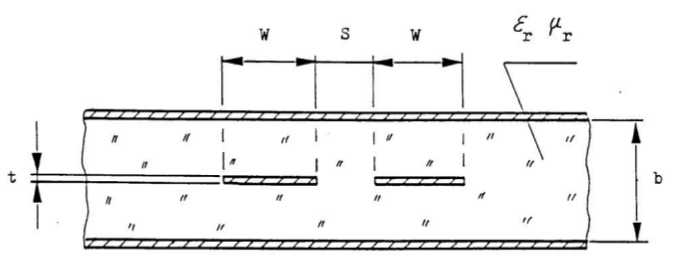
\includegraphics[scale=0.5]{fig/zad8/cstripline}
  \caption{Symetryczne linie paskowe}
  \label{fig:zad8:cstripline}
\end{figure}

\section{Rozwiązanie}
Impedancje charakterystyczne symetrycznych sprzężonych linii paskowych wynoszą:
\begin{align}
  Z_{0e} &= 29.976 \pi \sqrt{\frac{\mu_r}{\epsilon_r}}\frac{K'(ke)}{K(ke)} \\
  Z_{0o} &= 29.976 \pi \sqrt{\frac{\mu_r}{\epsilon_r}}\frac{K'(ko)}{K(ko)}
\end{align}
Powyższe wzory są słuszne gdy $t << b$,
co jest spełnione dla $t \approx 0$ określonego w zadaniu.

W pierwszym kroku należy wyznaczyć:
\begin{align}
  \frac{K'(ke)}{K(ke)} &= Z_{0e} / 29.976 \pi \sqrt{\frac{\mu_r}{\epsilon_r}} \\
  \frac{K'(ko)}{K(ko)} &= Z_{0o} / 29.976 \pi \sqrt{\frac{\mu_r}{\epsilon_r}}
\end{align}
Z ilorazu całek eliptycznych można wyznaczyć moduły~$k_e$ i~$k_o$.
Następnie obliczamy parametry linii $W$ i $S$ zgodnie ze wzorami:
\begin{align}
  W &= \frac{2b}{\pi}\operatorname{arth}(\sqrt{k_ek_o}) \label{eqn:zad8:w} \\
  S &= \frac{2b}{\pi}\operatorname{arth}\Big(\frac{k_e}{k_o}\Big) - W \label{eqn:zad8:s}
\end{align}

Dla wartości podanych w treści zadania potrzebne parametry linii to $w = 1.95755230148~mm$ i $s = 0.384595243329~mm$. 
\end{document}
